\documentclass{standalone}
\usepackage[T1]{fontenc}
\usepackage[utf8]{inputenc}
\usepackage[usenames,dvipsnames]{xcolor}
\usepackage{tikz}
\usetikzlibrary{plotmarks}
\usetikzlibrary{shapes,snakes,arrows}
\begin{document}
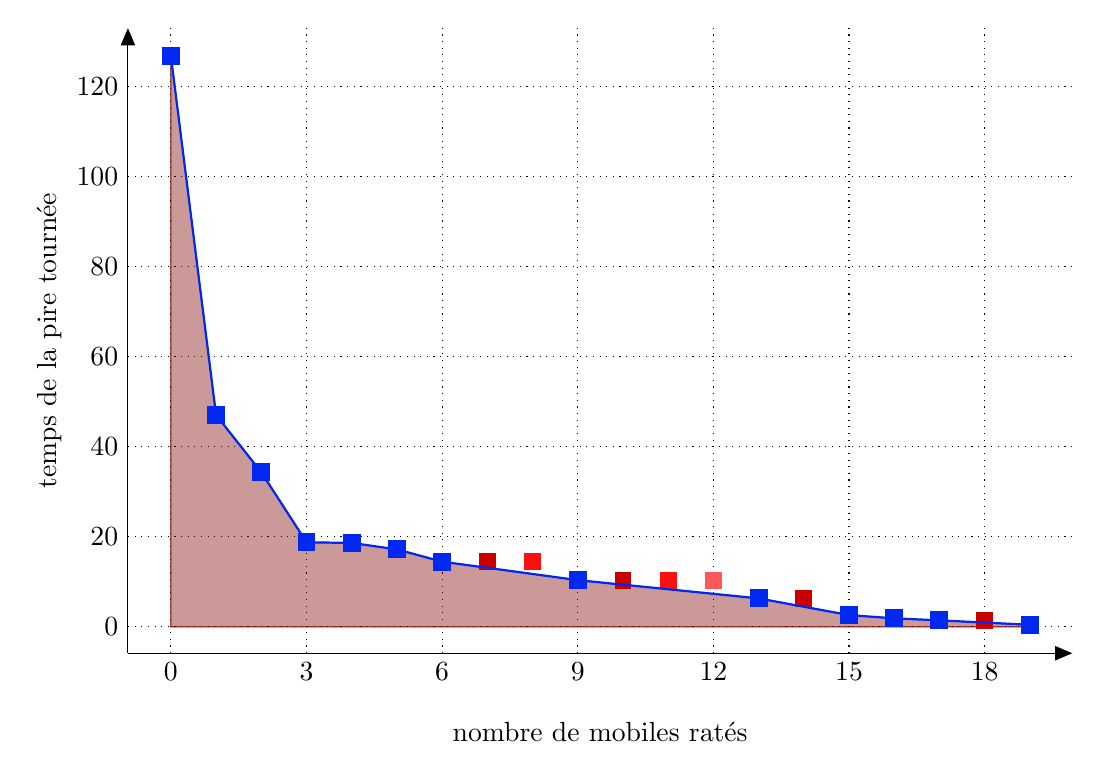
\begin{tikzpicture}[xscale=0.574163,yscale=0.057214]
\draw[xstep=3,ystep=20,thin,dotted,color=Black] (-0.95,-5.85439) grid (19.9383,132.868);
\begin{scope}
  \clip (-0.95,-5.85439) rectangle (19.9383,132.868);
  \definecolor{hvColor}{RGB}{128,0,0}
  \draw[color=hvColor, fill=hvColor, fill opacity=0.4] (0,0.458678) -- (0,126.72) -- (1,47.0057) -- (2,34.308) -- (3,18.7744) -- (4,18.631) -- (5,17.191) -- (6,14.4692) -- (9,10.3724) -- (13,6.32048) -- (15,2.61757) -- (16,1.8906) -- (17,1.44591) -- (19,0.458678) -| (19,0.458678) |- (0,0) -- cycle;
  \definecolor{pLineColor}{RGB}{200,0,0}
  \definecolor{pPointColor}{RGB}{200,0,0}
  \node[draw,color=pPointColor,fill=pPointColor, inner sep = 0pt, minimum size=2mm] at (7,14.4692) {};
  \node[draw,color=pPointColor,fill=pPointColor, inner sep = 0pt, minimum size=2mm] at (10,10.3724) {};
  \node[draw,color=pPointColor,fill=pPointColor, inner sep = 0pt, minimum size=2mm] at (14,6.32048) {};
  \node[draw,color=pPointColor,fill=pPointColor, inner sep = 0pt, minimum size=2mm] at (18,1.44591) {};
  \definecolor{pLineColor}{RGB}{255,16,16}
  \definecolor{pPointColor}{RGB}{255,16,16}
  \node[draw,color=pPointColor,fill=pPointColor, inner sep = 0pt, minimum size=2mm] at (8,14.4692) {};
  \node[draw,color=pPointColor,fill=pPointColor, inner sep = 0pt, minimum size=2mm] at (11,10.3724) {};
  \definecolor{pLineColor}{RGB}{255,88,88}
  \definecolor{pPointColor}{RGB}{255,88,88}
  \node[draw,color=pPointColor,fill=pPointColor, inner sep = 0pt, minimum size=2mm] at (12,10.3724) {};
  \definecolor{pLineColor}{RGB}{128,0,0}
  \definecolor{pPointColor}{RGB}{0,40,240}
  \draw[thick,color=pPointColor] (0,126.72) node[draw,color=pPointColor,fill=pPointColor, inner sep = 0pt, minimum size=2mm] {} -- (1,47.0057) node[draw,color=pPointColor,fill=pPointColor, inner sep = 0pt, minimum size=2mm] {} -- (2,34.308) node[draw,color=pPointColor,fill=pPointColor, inner sep = 0pt, minimum size=2mm] {} -- (3,18.7744) node[draw,color=pPointColor,fill=pPointColor, inner sep = 0pt, minimum size=2mm] {} -- (4,18.631) node[draw,color=pPointColor,fill=pPointColor, inner sep = 0pt, minimum size=2mm] {} -- (5,17.191) node[draw,color=pPointColor,fill=pPointColor, inner sep = 0pt, minimum size=2mm] {} -- (6,14.4692) node[draw,color=pPointColor,fill=pPointColor, inner sep = 0pt, minimum size=2mm] {} -- (9,10.3724) node[draw,color=pPointColor,fill=pPointColor, inner sep = 0pt, minimum size=2mm] {} -- (13,6.32048) node[draw,color=pPointColor,fill=pPointColor, inner sep = 0pt, minimum size=2mm] {} -- (15,2.61757) node[draw,color=pPointColor,fill=pPointColor, inner sep = 0pt, minimum size=2mm] {} -- (16,1.8906) node[draw,color=pPointColor,fill=pPointColor, inner sep = 0pt, minimum size=2mm] {} -- (17,1.44591) node[draw,color=pPointColor,fill=pPointColor, inner sep = 0pt, minimum size=2mm] {} -- (19,0.458678) node[draw,color=pPointColor,fill=pPointColor, inner sep = 0pt, minimum size=2mm] {};
\end{scope}
\draw[->,>=triangle 45] (-0.95,-5.85439) -- coordinate (x axis mid) (19.9383,-5.85439);
\node[below=1cm,anchor=center] at (x axis mid) {nombre de mobiles ratés};
\foreach \x in {0,3,6,9,12,15,18}
  \draw (\x,-5.85439) -- (\x,-5.85439) node[anchor=north] {\x};
\draw[->,>=triangle 45] (-0.95,-5.85439) -- coordinate (y axis mid) (-0.95,132.868);
\node[left=1cm,rotate=90,anchor=center] at (y axis mid) {temps de la pire tournée};
\foreach \y in {0,20,40,60,80,100,120}
  \draw (-0.95,\y) -- (-0.95,\y) node[anchor=east] {\y};
\end{tikzpicture}
\end{document}
